\documentclass[10pt,letter]{article}
	% basic article document class
	% use percent signs to make comments to yourself -- they will not show up.

\usepackage{amsmath}
\usepackage{amssymb}
	% packages that allow mathematical formatting

\usepackage{graphicx}
	% package that allows you to include graphics

\usepackage{setspace}
	% package that allows you to change spacing

\onehalfspacing
	% text become 1.5 spaced

\usepackage{fullpage}
	% package that specifies normal margins
	
\usepackage[version=3]{mhchem} % Package for chemical equation typesetting
\usepackage{graphicx} % Required for the inclusion of images
\usepackage{natbib} % Required to change bibliography style to APA
\usepackage{amsmath} % Required for some math elements 
\usepackage{booktabs}
\usepackage{floatrow}
	

\begin{document}
	% line of code telling latex that your document is beginning


\title{CS 156 Problem Set 5}

\author{Christopher Zhen}

\date{Oct 31, 2016}
	% Note: when you omit this command, the current dateis automatically included
 
\maketitle 
	% tells latex to follow your header (e.g., title, author) commands.

\section*{Problem 1}

\textbf{(C)} - We can solve for the smallest possible possible value of N by solving the following equation:

\begin{align*}
\mathbb{E}_\mathcal{D}[E_\textrm{in}(\boldsymbol{w}_\textrm{ln})] & = \sigma^2(1 - \frac{d+1}{N}) \\
0.008 & = (0.1)^2(1 - \frac{(8)+1}{N}) \\
N & = 45
\end{align*}

So the lowest answer choice that satisfies the desired expected in-sample error is $N = 100$.

\section*{Problem 2}

\textbf{(D)} - To achieve the desired boundary, we can use the following formula of a hyperbola:

\begin{align*}
ax_1^2 - bx_2^2 & = 1 \\
ax_1^2 - bx_2^2 -1 & = 0 \\
\end{align*}

However, because this equation gives the opposite dichotomy as the one desired, we need to multiply everything by -1 to get:

\begin{align*}
-ax_1^2 + bx_2^2 +1 & = 0 \\
\end{align*}

Which matches with answer choice D.

%\begin{figure}[H]
%\begin{center}
%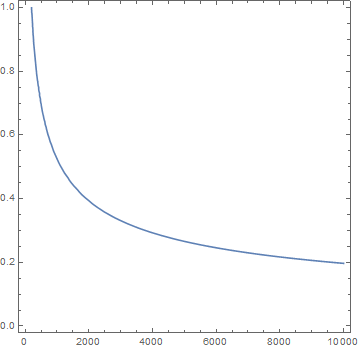
\includegraphics[width=0.5\textwidth]{2d.png}
%\caption{Table courtesy of the textbook %textit{Learning from Data}.}
%\label{2d}
%\end{center}
%\end{figure}

\section*{Problem 3} 

\textbf{(C)} - The Devroye bound this time is around 2 at $N=5$ while the Parrond bound is around 1.7.

\section*{Problem 4}

\textbf{(E)} - The code outputs an $\hat{a} = 1.45$ which doesn't match any of the options. 

\section*{Problem 5}

\textbf{(B)} - The code outputs 0.28 which is closest to 0.3. It makes sense for the bias in this case to be slightly worse than the $\bar{g}(x) = ax+b$ case from class, but better than the $\bar{g}(x) = b$ case.

\section*{Problem 6}

\textbf{(A)} - The code outputs a value of 0.24 which is closest to 0.2. It makes sense for this method to have smaller variances because there will never be negative values for \^{a} and the value at $x=0$ will always be the same.

\section*{Problem 7}

\textbf{(B)} - In lecture, we already derived the expected value using the bias-variance approach of both (A) and (C) and found that they were 0.75 and 1.90 respectively. The calculated value for (B) is  0.52 which is lower than both. Intuitively, since both (D) and (E) are even functions and we're fitting an odd function, neither should have a lower error than the other 3 functions, leaving (B) as the best choice.

\section*{Problem 8}

\textbf{(C)} - Since $m_\mathcal{H}(1) = 2$ and $m_\mathcal{H}(N+1) = 2 m_\mathcal{H}(N) - a$ (where a is some value), we'll always have the case where $m_\mathcal{H}(N) = 2^N$ for any value where a is 0. The value of a is only non-zero when $q \leq N$, so our first non-zero value will occur when $N = q$ and our VC dimension is $q$.

\section*{Problem 9}

\textbf{(B)} - Consider the concrete example of perceptrons. If our hypothesis sets are the different dimensions of perceptrons, the maximum VC dimension of our intersection is simply the maximum VC dimension of the highest dimension perceptron. The minimum is then just the case where the intersection is 0.

\section*{Problem 10}

\textbf{(E)} - The answer must be D or E because the union of sets contains the hypothesis with the highest dimension, so the dimension of the union must at least be the maximum VC dimension of a single set. Now consider the case where we have a VC dimension of 0. In this case, the growth function is bounded by: 

\begin{align*}
m_\mathcal{H} & = \sum_{i=0}^{d_{\textrm{vc}}}\binom Ni \\
m_\mathcal{H} & = N^{d_{\textrm{vc}}} + 1 \\
m_\mathcal{H} & = 1 \\
\end{align*}

So the max VC dimension has to include a term to account for the case where we have up to K hypotheses with a VC dimension of 0 by adding on K-1 (since when K = 1, the VC dimension is still 0).

\end{document}
	% line of code telling latex that your document is ending. If you leave this out, you'll get an error
